%\documentclass[11pt,a4paper,twoside,openright]{report}
\documentclass[11pt,a4paper]{report}

\def\b0{{\bf 0}}
\def\ba{{\bf a}}
\def\bb{{\bf b}}
\def\bc{{\bf c}}
\def\bd{{\bf d}}
\def\be{{\bf e}}
\def\bg{{\bf g}}
\def\bh{{\bf h}}
\def\bi{{\bf i}}
\def\bj{{\bf j}}
\def\bk{{\bf k}}
\def\bl{{\bf l}}
\def\bm{{\bf m}}
\def\bn{{\bf n}}
\def\bo{{\bf o}}
\def\bp{{\bf p}}
\def\bq{{\bf q}}
\def\br{{\bf r}}
\def\bs{{\bf s}}
\def\bt{{\bf t}}
\def\bu{{\bf u}}
\def\bv{{\bf v}}
\def\bw{{\bf w}}
\def\bx{{\bf x}}
\def\by{{\bf y}}
\def\bz{{\bf z}}

\def\bSigma{{\bf \Sigma}}
\def\bA{{\bf A}}
\def\bB{{\bf B}}
\def\bC{{\bf C}}
\def\bD{{\bf D}}
\def\bE{{\bf E}}
\def\bF{{\bf F}}
\def\bG{{\bf G}}
\def\bH{{\bf H}}
\def\bI{{\bf I}}
\def\bJ{{\bf J}}
\def\bK{{\bf K}}
\def\bL{{\bf L}}
\def\bM{{\bf M}}
\def\bN{{\bf N}}
\def\bO{{\bf O}}
\def\bP{{\bf P}}
\def\bQ{{\bf Q}}
\def\bR{{\bf R}}
\def\bS{{\bf S}}
\def\bT{{\bf T}}
\def\bU{{\bf U}}
\def\bV{{\bf V}}
\def\bW{{\bf W}}
\def\bX{{\bf X}}
\def\bY{{\bf Y}}
\def\bZ{{\bf Z}}
\def\imwidth{0.60}

\usepackage{anysize}
\usepackage{iitbtitle}   %% For Thesis Title Page with IITB Logo
\usepackage{latexsym}
\usepackage{pictex}
\usepackage{fancyvrb}
\usepackage{fancyhdr}
\usepackage{color}
\usepackage{graphicx}
% \usepackage{subfigure}
\usepackage{rawfonts}
\usepackage{amssymb}
\usepackage{amsmath}
\usepackage{mathtools}
% \usepackage{caption}
\usepackage{subcaption}

\DeclarePairedDelimiter\floor{\lfloor}{\rfloor}
%\usepackage{hyperref}
%\usepackage{newcent} %the options are:  palatino, times, newcent, bookman

\marginsize{1.5in}{1in}{0.75in}{0.75in}
% \renewcommand\baselinestretch{1}

\newif\ifpdf
\ifx\pdfoutput\undefined
    \pdffalse           % we are not running PDFLaTeX
\else
    \pdfoutput=1        % we are running PDFLaTeX
    \pdftrue
\fi


\ifpdf
\usepackage[pdftex,
        colorlinks=true,
        urlcolor=black,       % \href{...}{...} external (URL)
        filecolor=black,     % \href{...} local file
        linkcolor=black,       % \ref{...} and \pageref{...}
	citecolor=black,
        pdftitle={Dual Degree. Thesis},
        pdfauthor={Mohit Madan},
        % pdfsubject={Variational Parametric Models for Audio Synthesis},
        % pdfkeywords={Generative Synthesis, Parametric Models},
%        pagebackref,
%        pdfpagemode=true,
        bookmarksopen=true]{hyperref}
\pdfcompresslevel=9
\else
%    \usepackage[ps2pdf,
%        colorlinks=true,
%        urlcolor=black,               % \href{...}{...}
%        anchorcolor=black,
%        filecolor=black,             % \href*{...}
%        linkcolor=black,               % \ref{...} and \pageref{...}
%        menucolor=black,
%        citecolor=black]{hyperref}
    \usepackage{hyperref}
    \usepackage{graphicx}
\fi

%\definecolor{rltbrightred}{rgb}{1,0,0}
%\definecolor{rltred}{rgb}{0.75,0,0}
%\definecolor{rltdarkred}{rgb}{0.5,0,0}
%%
%\definecolor{rltbrightgreen}{rgb}{0,0.75,0}
%\definecolor{rltgreen}{rgb}{0,0.5,0}
%\definecolor{rltdarkgreen}{rgb}{0,0,0.25}
%%
%\definecolor{rltbrightblue}{rgb}{0,0,1}
%\definecolor{rltblue}{rgb}{0,0,0.75}
%\definecolor{rltdarkblue}{rgb}{0,0,0.5}
%
%\definecolor{webred}{rgb}{0.5,.25,0}
%\definecolor{webblue}{rgb}{0,0,0.75}
%\definecolor{webgreen}{rgb}{0,0.5,0}



% \title{Limited CSI feedback for MIMO-OFDM channel}
% \author{Mohit Madan}
% \date{2020}

\begin{document}
\def\title{Limited CSI feedback for MIMO-OFDM channel}
\def\what{Dissertation}
\def\degree{Bachelor \& Master~of~Technology}
\def\who{Mohit Madan}
\def\roll{15D070028}
\def\guide{Prof. Kumar Appaiah}
\def\dept{Department of Electrical Engineering}
\def\year{2020}
\pagenumbering{roman}

%\ifpdf
%\pdfbookmark[1]{Title}{title} %%This is pdf specefic
%\fi
\iitbtitlepage

% Approval, edit approval.tex
\thispagestyle{empty}
\begin{center} \label{chap:approval}
{\Large \bf { Dissertation Approval Sheet}} \\
\vspace{0.4in}
This is to certify that the dissertation titled\\
\vspace{0.1in}
{\bf \title} \\
\vspace{0.2in}
 By \\
\vspace{0.2in}
{\bf \who} \\ (\roll) \\
\vspace{0.2in}
is approved for the degree of {\bf \degree}.\\
\vspace{0.8in}
\line(1,0){200}\\
{ \guide } \\
{ (Guide)} \\
%\vspace{0.8in}
%\line(1,0){200}\\
%{ \coguide } \\
%{ (Co-Guide)} \\
\vspace{0.8in}
\line(1,0){200}\\
{ Internal Examiner} \\
\vspace{0.8in}
\line(1,0){200}\\
{ External Examiner} \\
\vspace{0.8in}
\line(1,0){200}\\
{ Chairperson} \\
\end{center}
\vspace*{0.3in}
\noindent {Date : } \line(1,0){100}
\newpage
%%


% Declaration, edit declaration.tex
% \thispagestyle{empty}
\label{chap:declaration}
\begin{center}
{\Large \bf { Declaration of Authorship}}
\end{center}
\vspace{0.4in}

I, {\bf \who} declare that this written submission represents my ideas in my own words and where others
ideas or words have been included, I have adequately cited and referenced the original sources.
I also declare that I have adhered to all principles of academic honesty and integrity and have
not misrepresented or fabricated or falsified any idea/data/fact/source in my submission. I
understand that any violation of the above will be cause for disciplinary action by the Institute
and can also evoke penal action from the sources which have thus not been properly cited or
from whom proper permission has not been taken when needed.


\vspace{0.2in}

\begin{flushright}
\hfill
\line(1,0){200}
\newline
\hfill{Signature}
\end{flushright}

\vspace{0.1in}

\begin{flushright}
\hfill
\line(1,0){200}
\newline
\hfill{Roll Number}
\end{flushright}

\vspace{0.1in}

\begin{flushleft}
{Date: }\line(1,0){100} \hfill
\end{flushleft}


% Abstract, edit abstract.tex
%%---------------- A B S T R A C T -----------------
\vspace*{2in}
\section*{\begin{center} {\Huge{Abstract}}\end{center}}
%\thispagestyle{empty}
\addcontentsline{toc}{chapter}{\quad\,\,{Abstract}}

In MIMO-OFDM systems or any other wireless chanels, channel adaptive techniques
result in improvement of channel capacity and obtains lower
Bit error rates. Unfortunately, this has been impractical in the past 
due to unavailability of the channel state information (CSI) at the transmitter.
A lot of reasearch has been done over the years to obtain channel knowledge at
the transmitter by using the feed back from the receiver side. 
CSI has to be estimated at the receiver and then it is quantized and fed back 
to the transmitter. However, due to larger number of subcarriers in case of OFDM
systems along with increasing number of transmitter antennas, the total size of the 
feedback becomes very large. 
Therefore, there is a need to compress and quantize the CSI before it is fed back. 
We propose a framework using Given's rotation for adaptive quantization and 
feedback of channel knowledge and then compare its performance with the existing 
solutions especially manifold based approaches.
Moreover, we also see how feedback changes and how the existing method is modified as 
the number of transmitter antennas increases.

% The MIMO and massive MIMO wireless channels offer great capacities
% and gains as compared to channels with fewer transmitter and recceiver
% antennas. This gain is made possible due to the increased diversity
% and degrees of freedom in the channel. Channel state information plays
% a huge role in achieving this gain by making beamforming and waterfilling
% possible at the transmitter. 
% Channel is estimated at the receiver  

% In MIMO wireless channel state information is at the transmitter


% Acknowledgement, edit ack.tex
% \section*{\begin{center}\Huge{Acknowledgments}\end{center}}
%\thispagestyle{empty}
\addcontentsline{toc}{chapter}{\quad\,\,{Acknowledgments}}
\indent I express my sincere gratitude towards my guide \textbf{\guide} and
%\textbf{\coguide} for their constant help, encouragement and inspiration
throughout the project work. 

\vspace{1in}\noindent
\begin{flushright}
\textbf{\who}\\
IIT Bombay\\
(Date)
\end{flushright}



%-----------------Table of Contents-------------------
%\renewcommand{\tableofcontents}{Table of Contents}
\newpage
%\ifpdf
\pdfbookmark[0]{Table of Contents}{contents} %%This is pdf specefic
%\fi
%\addcontentsline{toc}{chapter}{\quad\,\,{Contents}}
\tableofcontents
%\thispagestyle{empty} 
%\addtocontents{toc}{\protect\thispagestyle{empty}} 
\newpage

% \listoffigures
%\thispagestyle{empty} 
\addcontentsline{toc}{chapter}{\quad\,\,{List of Figures}}
%\addtocontents{lof}{\protect\thispagestyle{empty}} 
%\newpage


%-------Chapter Headings--------
\pagestyle{fancy}
\fancyhead[LE]{\leftmark}
\fancyhead[LO]{}
\fancyhead[RO]{\rightmark}
\fancyhead[RE]{}
\fancyfoot[C]{\thepage}
\renewcommand{\headrulewidth}{0.1pt}
\renewcommand{\footrulewidth}{0pt}

\renewcommand{\sectionmark}[1]{%
\markright{\it \thesection \ #1}{}}

\renewcommand{\chaptermark}[1]{%
\markboth{\it \chaptername \ \thechapter.\ #1}{}}

% Arabic Numbering for Chapters
%--------------------------------------- Chapter 1 ------------------------------------
\chapter{Introduction: MIMO OFDM wireless channel}
\label{chap:intro}
\pagenumbering{arabic}

\section{Introduction to MIMO wireless channels}
Multiple-Input Multiple-Output (MIMO) is a technology which uses multiple antennas 
at transmitter and receivers to increase the data rate. All wireless products using 
the technology 802.11n and onwards use MIMO to provide higher gains.
Multiple-Input Multiple-Output orthogonal frequency division multiplexing (MIMO-OFDM)
is an interface which is used for 4G and 5G wireless communication. OFDM divides a 
a frequency selective channel into a group of orthogonal flat fading sub-channels, which
provides more reliable communication at higher speeds. 

The innovation that has helped to overcome the challenge of making instantaneous
channel adaptation practical is the use of feedback of Channel State Information 
(CSI) is known at the Transmitter (CSIT). This information provides information
about the forward link condition which is then used by the transmitters to 
adapt to the forward link transmission.

\section{Channel State Information}     
CSI is estimated at the receiver using estimation techniques like Least Square (LS)
and Minimum Mean Square Error (MMSE) estimation. For estimation, pilot symbols
(known at the receiver) are send by the transmitter, which are then used to estimate
the channel at the receiver.

One key requirement to achieve the channel capacity is to leverage spacial multiplexing gains
obtained by precoding transmissions by Singular Value Decomposition (SVD) of the MIMO
channel matrix~\cite{love2008overview}. However, this requires the receiver to
feed back the unitary matrix obtained by the SVD, to the transmitter.

With increasing the number of subcarriers in OFDM channels or with 
increasing number of antennas with MIMO, there is a need to provide
feedback in a limited sense.

\begin{figure}
\begin{center}
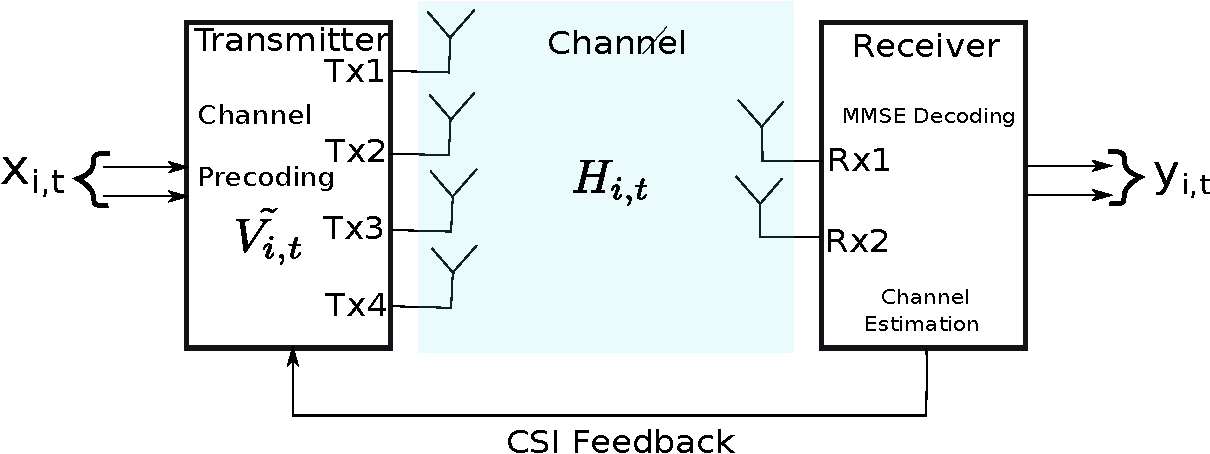
\includegraphics[width=0.9\columnwidth]{images/drawing.pdf}
\caption{Figure shows a $4\times2$ MIMO channel. Here $x_{i,t}$ is the input vector
which is then precoded using $V_{i,t}$ and then sent over a channel H after
doing necessary processing at the transmitter. It is then recovered at the receiver using
MMSE decoding. Channel is estimated using estimation techniques and precoder is fed back to the
transmitter. }
\label{fig:mimo}
\end{center}
\end{figure}

\section{Thesis Objective and Scope}
To reduce the feedback overhead, past work taps in the inherent temporal and frequency correlations in SVD precoders, in order to perform effective quantization with just a few bits by utilizing predictive quantization \cite{Gupt1905:Predictive,6891198,7370793,sacristan2010differential,5946308,6545375,4114278,4556174}, and reducing number of fed back subcarriers by utilizing interpolation algorithms \cite{Gupt1905:Predictive,5671092,khaled2005quantized}.

An underlying challenge in framing the predictive quantization and interpolation algorithms has been the high dimensional unitary structure of the SVD precoders. A large body of work utilizes the manifold geometry endowed by the unitary structure to frame such algorithms directly on the non-linear manifold ~\cite{schwarz2013adaptive,5946308,6891198,Gupt1905:Predictive,pitaval2013codebooks}. On the other hand, there are numerous works which utilize scalar parameterization of the unitary precoders, given by Givens rotations and Householder transformations \cite{4114278,4556174,lou2013comparison}. While the manifold based methods offer a clean solution and have been shown to be very effective in reducing the feedback overhead, they are analytically terse and
involve operations over higher dimensional manifolds. The scalar parameterization algorithms enable usage of the traditional algorithms to predict, interpolate and quantize over vector spaces, and hence are analytically simpler.
Such methods have also been implemented in 802.11 ac and ax standards
\cite{lou2013comparison,ieee80211}. We are not aware of performance comparisons
between these two bodies of work, thereby making it difficult to
quantify from past work whether performance gains/losses can accrue by operating over scalar parameterization instead of manifolds.

This work aims at designing a framework for an effective method for CSI quantization
and feedback which help to realize lower BER rates and higher capacities. The scope 
of this work is limited to effective feedback and considers all other parameters
ideal i.e. the channel estimation at receiver is considered to be perfect. Simulations
are performed over various practical channel models using sufficiently large amount
of data in order to verify the claims.
\section{Thesis Outline}
In second chapter we discuss about the channel model and performance analysis. 
In Third Chapter we discuss about the scalar joint-time frequency interpolation
scheme and in the fourth chapter about the capacity calculation with and 
without channel knowledge and effect of number of transmitters on channel capacity.
Finally, thesis ends with the conclusion and the scope of the future work.

% \section{TODO}
% % add figures of MIMO and MIMO OFDM.
% Take more information from introduction and
% explain about manifold method and how it is compared.
% Talk about how capacity is increased by using the notes from the google docs and
% the book. Site book also if necessary or try to redraw figures from there.
% Include the Bibliography .bib file here, the style can be changed as well


\chapter{System Model}
\label{chap:sysMod}

\section{Channel}
For a MIMO-OFDM system with $N_T$ transmitter and $N_R$
receiver antennas, the channel for the $\emph{i-th}$ subcarrier at time
instant $\emph{t}$ can be modeled as a flat-fading MIMO channel. This
flat-fading MIMO channel can be written as

\begin{equation}
% \label{section2}
\by_{i,t} = \bH_{i,t}\tilde{\bV}_{i,t} \bx_{i,t}+ {\boldsymbol{\eta}}_{i,t}
\end{equation}
where $\bH_{i,t} \in {\mathbb{C}}^{N_R \times N_T}$ is the channel
matrix, $\bx_{i,t} \in {\mathbb{C}}^{N_d}$ is the input data vector,
$\by_{i,t} \in {\mathbb{C}}^{N_R}$ is the output vector,
$\tilde{\bV}_{i,t} \in {\mathbb{C}}^{N_T \times N_R}$ is the unitary
precoder, and $\bf{\eta}$ is the complex additive white Gaussian noise
distributed as ${\mathcal{CN}}(0,I_{N_R})$. We consider the case where
$N_R < N_T$, and the data vector size $N_d = N_R$.  The ``thin'' SVD
(which keeps only those right and left singular vectors that correspond
to non-zero singular values) of $\bH$ is given by

\begin{equation}
\bH_{i,t} = \bU_{i,t} \bSigma_{i,t} \bV_{i,t}^{H}
\end{equation}
where $\bU_{i,t} \in \mathbb{C}^{N_R \times N_R}$,
$\bSigma_{i,t} \in \mathbb{C}^{N_R \times N_R}$ and
$\bV_{i,t} \in \mathbb{C}^{N_T \times N_R}$. $\bU_{i,t}$ and
$\bV_{i,t}$ are matrices whose columns are orthonormal, and
$\bSigma_{i,t}$ contains the singular values
$\sigma_1 \geq \ldots \geq \sigma_{N_R} > 0$ of $\bH_{i,t}$. The
entries of $\bH_{i,t}$ are assumed to be distributed
i.i.d. $\mathcal{CN}(0,1)$. To obtain a precoder at the
transmitter, we need to quantize and feed back information about
$\bV_{i,t}$ for each subcarrier. However, the frequency coherence and
temporal correlations would reduce the overall feedback requirement,
as discussed in subsequent sections.

% \section{Performance Analysis}
% \label{sec:cap}
% In current frequency division duplexing (FDD) MIMO systems the forward
% and reverse links generally have highly uncorrelated channels because
% they are separated in frequency.

\chapter{Scalar Joint-Time frequency precoder feedback scheme}
\label{chap:scheme}

\section{Scheme}
The orthonormal precoder matrices $\tilde{\bV}_{i,t}$ which need to be fed back
to the transmitter are decomposed into minimal scalar components using
Givens Rotation method. This method iteratively breaks down an orthonormal
complex matrix into its independent scalar components/angles
($\bf{\Theta}$s and $\bf{\Phi}$s) as given in Section~\ref{sec:param}. 
These parameters are then quantized using B bits for the first time instant 
for only few subcarriers which are going to be fed back and tracked as given 
in Section~\ref{sec:quant}. These parameters for the limited subcarriers are 
then tracked for the later time instances using differential quantization scheme
as given in Section~\ref{sec:track}. 
After obtaining the quantized parameters for the limited precoders obtained
at the transmitter, the parameters are interpolated for the rest of the unsent
precoders as given in Section~\ref{sec:interp}. These parameters are then used 
to obtain the precoder back using an inverse of the Givens decomposition method. 

\section{Scalar Parameterization using Givens Rotation}
\label{sec:param}
The degrees of freedom in the precoder matrix $\tilde{\bV}_{i,t}$ is
smaller than the total number of real entries in the matrix because of 
the orthogonality between the columns of the matrix~\cite{4114278}.
Therefore, this orthogonality could be used to paramaterize $\tilde{\bV}_{i,t}$ 
using fewer parameters than the total number of real entries in the matrix.

The orthonormal matrix $\tilde{\bV}_{i,t}$ with $N_T$ rows and $N_R$ columns
can be decomposed using Givens rotation as follows:
\begin{equation}
\label{eq:decompose}
\tilde{\bV}_{i,t} = \left[\prod_{k=1}^{N_{R}} \bD_{k} \left( \phi_{k,k},\ldots , \phi_{k,N_{R}} \right) \:  \prod_{l=1}^{N_{T}-k} \bG_{N_{T}-l,N_{T} -l+1} \big( \theta_{k,l}\big)  \right] \: \tilde{\bI}
\end{equation}
where $\bD_{k}$ is a diagonal matrix defined as
$\bD_{k}\big(\phi_{k,k}, \ldots, \phi_{k,N_T } \big)$ =
$\mbox{diag}\big( {\bf 1}_{k-1}, e^{j\phi_{k,k}},\ldots,
e^{j\phi_{k,N_T }} \big)$ with  dimension $N_T \times N_T$. ${\bf 1}_{k-1}$ represents $k-1$ ones,
and the $N_T \times N_R$ matrix $\tilde{\bI}$ =
$\big[\bI_{N_R }, {\bf 0}_{N_R ,N_T -N_R}\big]^{T}$. Here,
${\bf 0}_{N_R ,N_T -N_R }$ is an $N_R\times (N_T - N_R)$ matrix all of
whose elements are zero.
Finally $\bG_{m-1,m}\big(\theta\big)$ is a matrix with dimension $N_T \times N_T$ and is given as follows:
\begin{equation}
\bG_{m-1,m}\big(\theta\big)  =
\begin{bmatrix}
\bI_{m-2} & & & \\
& \cos\theta & -\sin\theta & \\
& \sin\theta & \cos\theta & \\
& & & \bI_{N_T -m}
\end{bmatrix}
\end{equation}

Above parameterization is clarified with an example. Consider a $4 \times 2$ 
orthonormal matrix $\tilde{\bV}_{i,t}$ as:

\begin{equation}
\label{eq:example}
\tilde{\bV}_{i,t} = 
\begin{bmatrix}
\times & \times \\
\times & \times \\
\times & \times \\
\times & \times \\
\end{bmatrix}
\xrightarrow{\text{$\bD^{\dagger}_1$}}
\begin{bmatrix}
|\times| & \times \\
|\times| & \times \\
|\times| & \times \\
|\times| & \times \\
\end{bmatrix}
\xrightarrow{\text{$\bG^{\dagger}_{3,4} , \bG^{\dagger}_{2,3}, \bG^{\dagger}_{1,2}$}}
\begin{bmatrix}
1 & 0 \\
0 & \times \\
0 & \times \\
0 & \times \\
\end{bmatrix}
\xrightarrow{\text{$\bD^{\dagger}_2$}}
\begin{bmatrix}
1 & 0 \\
0 & |\times| \\
0 & |\times| \\
0 & |\times| \\
\end{bmatrix}
\xrightarrow{\text{$\bG^{\dagger}_{3,4} , \bG^{\dagger}_{2,3}$}}
\tilde{\emph{\bI}}
\end{equation}
In the equation above, $|\times|$ denotes the magnitude of a 
particular element. In the first step, we want to make all the entries
in the first column under the first element to become zero. To do that,
we extract the phases from the first column by pre-multiply $\tilde{\bV}_{i,t}$
by a matrix $\bD^{\dagger}_1$ to make the first column real. Then we pre-multiply
by a series of Givens matrices to make all the elements under the element (1,1)
to be zero. Since the Givens rotation operation preserves the length of the 
of a vector, the (1,1) element becomes 1. Also, because of the orthogonality of
the column vectors, all the elements except (1,1) in the first row
becomes 0. This procedure is followed iteratively for the remaining columns
until $\tilde{bI}$ is obtained finally. Thus a $4\times2$ orthonormal
matrix $\tilde{\bV}_{i,t}$ can be decomposed using Givens rotation matrices
as follows:
\begin{equation}
  \bV_{i,t}  =
  \bD_{1}(\phi_{1,1},\ldots,\phi_{1,4})\bG_{3,4}(\theta_{1,1})
  \bG_{2,3}(\theta_{1,2}) \bG_{1,2}(\theta_{1,3})
  \bD_{2}(\phi_{2,2},\phi_{2,3},\phi_{2,4}) \bG_{3,4}(\theta_{2,1}) \bG_{2,3}(\theta_{2,2})\tilde{\bI}
\end{equation}
Here, $\phi_{k,l}$s are referred to as phases, and their collection
for the $i$-th subcarrier at time instant $t$ is captured in a vector
denoted by $\bf{\Phi}$$_{i,t}$.
\begin{figure}
\begin{center}
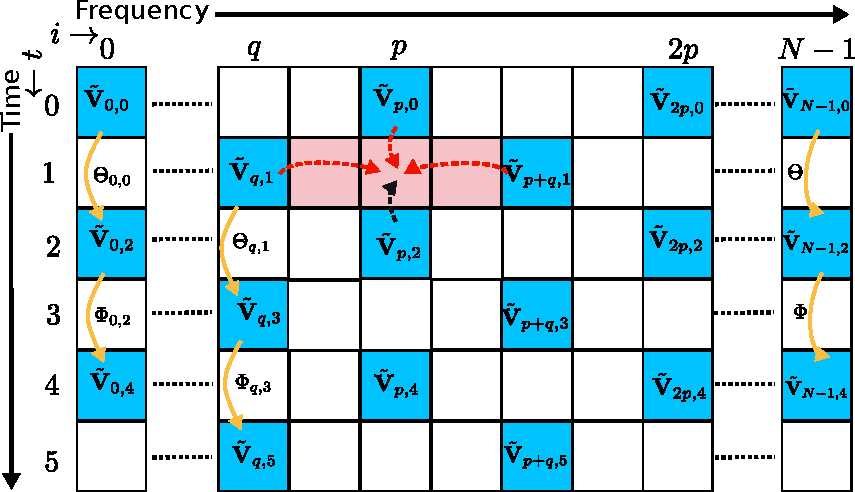
\includegraphics[width=0.7\columnwidth]{images/new-adpm2.pdf}
\caption{\label{fig:adpm-fig}Subcarriers that need to be
  quantized. Subcarriers indicated by red shaded cells have precoders 
  whose parameters are determined using the neighbouring parameters
  (shown via red arrows), both in time and frequency. The black arrow 
  indicates refinement of past precoders as fresher estimates are made
  available.}
\end{center}
\end{figure}
$\theta_{k,l}$s are called rotation angles, and their collection is
captured in a vector referred to as $\bf{\Theta}$$_{i,t}$. We note that
$\bf{\Phi}$$_{i,t}$ and $\bf{\Theta}$$_{i,t}$ represent the phase and
rotation angles for the $i$-th subcarrier at time instant $t$, as
represented in Fig.~\ref{fig:adpm-fig}. It is known
that $\phi_{k,l} \in (-\pi, \pi]$ for all k and l's is uniformly
distributed between the two extremes~\cite{4114278}, while
$\theta_{k,l}$ is distributed as
\begin{equation}
2l(\sin\theta_{k,l})^{2l-1}\cos\theta_{k,l}, for \;
\theta_{k,l} \in \left[0,\: \frac{\pi}{2}\right),\: 1\leq k \leq N_R,
1\leq l \leq N_T -k
\end{equation}
The total number of parameters obtained from the
decomposition of a complex orthogonal matrix $N_{T} \times N_{R} $ is
$N_{R}(2N_{T} - N_{R})$. The number of $\phi_{k,l}$ parameters is
$N_{R}(2N_{T} - N_{R}+1)/2$ while the number of $\theta_{k,l}$
parameters is $N_{R}(2N_{T} - N_{R}-1)/2$. Thus, ${\bf{\Phi}}_{i,t}$
is a vector of length $N_{R}(2N_{T} - N_{R}+1)/2$, while
${\bf{\Theta}}_{i,t}$ has length
$N_{R}(2N_{T} - N_{R}-1)/2$.~\cite{4114278}

The parameterization approach described above is related
to the channel state information feedback present in several
wireless standards, including 802.11ac~\cite{lou2013comparison}, 
although adaptive quantization and feedback are not discussed. 
Further sections show that the use of adaptive approaches can 
greatly enhance performance with only very minor modifications 
to the system.

\section{Quantization}
\label{sec:quant}
B bits each are used to quantize all $\theta_{k,l}$s and $\phi_{k,l}$s for the
initilization in the first time instant.
The distribution of the $\theta_{k,l}$ and $\phi_{k,l}$ is used to
quantize $\bf{\Theta}$ and $\bf{\Phi}$ respectively. 
Since, $\theta_k,l$ is distributed uniformly between 
$-\pi$ and $\pi$, therefore, the interval $(-\pi,\pi]$ is divided
uniformly into $2^B$ parts.

As $\Phi_k,l$ distribution is given, Lloyd's quantization~\cite{lloyd1982least} 
is used to divide $[0,\frac{\pi}{2})$ into $2^B$ optimal intervals. 
In addition, $\phi_{k,l}$ and
$\theta_{k,l}$ are statistically independent, making this
representation useful for tracking them separately across time, as
discussed below.

\section{Differential quantization and Channel tracking}
\label{sec:track}
For channels that vary slowly with time, adaptive differential
quantization is an effective method for tracking parameters over time
using very few bits (often just one bit per parameter). For example,
while tracking a slowly varying discrete random process $x_n$ at time
$n$, the one bit can be used to determine the direction in which to
move in order to track the parameter. This can be denoted by
$\beta_{n} = \mbox{sign}(x_{n} - \hat{x}_{n-1})$, where $x_n$ is the
unquantized (accurate) value and $\hat{x}_{n-1}$ is the quantized
value. Further, the step size for the move can be adapted based on the
speed of channel variation as well the accuracy needed. If $\Delta_n$
is the step size, we define our adaptive quantizer as
\begin{equation}
\hat{x}_{n} = \hat{x}_{n-1} + \beta_{n}\Delta_{n} \mbox{ where }
\label{delta_eqn}
\Delta_{n} = \begin{cases}
    M \Delta_{n-1}, & \text{if $\beta_{n} = \beta_{n-1}$}\\
    \Delta_{n-1}/M , & \text{if $\beta_{n} \neq \beta_{n-1}$}.
  \end{cases}
\end{equation}
where $M$ is the scaling factor used during the positive and negative
moves. We initialize $\Delta_1$ as $\Delta_1 = |x_{2}-\hat{x}_1|$. This is performed separately for each of the quantized
parameters.

To quantize the subcarriers efficiently and exploit the joint
time-frequency interpolation at the transmitter, we select the
subcarriers for quantization in an alternating fashion as shown in
Fig.~\ref{fig:adpm-fig}. The figure shows the channel evolution of an
$N$ subcarrier MIMO-OFDM system with the subcarriers that are
quantized. Every $p$-th subcarrier starting with $0$ is quantized for
even time instances, where, $p$ is the gap between two quantized
subcarrier indices. For odd time instances, subcarriers at the
position $pk+q$ for $k = 0,1,..., \frac{N-1}{p}$ with $q =
{\floor*{\frac{p}{2}}}$.

For the adaptive channel tracking scheme, the arrows in
Fig.~\ref{fig:adpm-fig} show how previous quantized values along with
the 1-bit enhancement are used to find the new quantized value. Since
we use a single bit adaptation, the amount of feedback required is 1
bit for each scalar parameter that is being tracked. On average, this
can be reduced by half if we transmit only $\bf{\Theta}$ values for
one-time instance and only $\bf{\Phi}$ values for the next time
instant in an alternating fashion (the untransmitted value is assumed
to be the same as that at the previous instant). In this case, the
average number of bits required to quantize a channel matrix will be
$N_{R}(2N_{T} - N_R )/2$ (from~\cite{4114278}). While tracking
the $\phi_{k,l}$ parameters, it must be noted they may change abruptly
between $-\pi$ and $\pi$ due to jumps of $2\pi$. This is avoided by
unwrapping the phases to facilitate continuous tracking (i.e., jumps
in phase of magnitude close to $2\pi$ have been eliminated).

\section{Joint Time Frequency Interpolation}
\label{sec:interp}
After obtaining the $\beta$ values (using the single bit feedback) at
the transmitter, we can construct the precoder at subcarrier indices
$pk$ or $pk+q$, keeping with the same notation as the previous
section.

In Fig.~\ref{fig:adpm-fig}, each parameter is interpolated using the
neighbouring subcarriers using bilinear interpolation (equivalent to
linear interpolation in two dimensions). These interpolated values are
then used to reconstruct the precoding matrices all together by
applying the reverse transformation of breaking the precoder into
independent parameters as given in
Equation~\ref{eq:decompose}. Precoder estimates are calculated using
the current and past data, though the earlier precoder estimates
are improved by refining the past estimates through
interpolation with current estimates (indicated by the black arrow in
Fig.~\ref{fig:adpm-fig}). Thus, the approach here is able to exploit
the time and frequency correlation jointly to enhance performance.

One reason why a linear predictive quantization is preferred is
because the underlying parameters can generally be thought to emerge
from an autoregressive (AR) process. For such processes, it is well
known that linear prediction based on past samples is optimal. Even
though the $\bf{\Theta}$ and $\bf{\Phi}$ parameters do not manifest as AR
processes, for small changes, a linear approximation works
sufficiently well, as described in~\cite{4114278}, although that
consideration was limited to tracking the temporal evolution of the
parameters.

\chapter{Optimal power allocation in MIMO systems}
\label{chap:cap}

\section{Channel Model}
\label{sec:1}
We consider a MIMO channel with i.i.d rayleigh fading model given as
\begin{equation}
\by = \bH\bx + \bn
\end{equation}
where H is channel matrix with shape $N_R\times N_T$ considering rayleigh flat-fading,
x is the transmit vector, y is the received vector and n is baseband
noise whose elements are zero-mean circularly-symmetric complex additive 
white Gaussian noise (AWGN) samples with variance of $\sigma^2$.
On keeping the number of receivers to a constant and varying the number of transmitter
antennas, it has been shown that at high SNR, waterfilling allocates
equal power P/$n_{min}$ to all the spatial modes, as well as equal amount
of power over time~\cite{10.5555/1111206}.
We will see the calculation of capacity in MIMO channel with and without
CSI knowledge at the transmitter and compare them later.

\subsection{Unknown CSI capacity at Transmitter}
When transmitter do not have knowledge of the underlying channel
then it is best to allocate total power P equally among all the 
transmitter antennas $N_T$. The capacity is given by~\cite{Foschini1998, Khalighi2002, 6770094} 
\begin{equation}
C = \sum_{i=1}^{N}log_{2}\big(1 + \frac{P}{N_{T}\sigma^2}\lambda^{2}_{H,i}\big)\: bits/s/Hz
\end{equation}
where $\lambda_{H,i}$ are singular values of the $\bH$ matrix and N = $min(N_T, N_R)$.
$\bH$ can be decomposed using SVD as $\bH = \bU\bSigma\bV^H$

\subsection{Known CSI capacity at Transmitter}
With channel knowledge at the transmitter, the power can be distributed
optimally over $N_T$ transmitter antennas inorder to achieve maximum
capacity. Using Lagrange multiplier, the capacity is given as
\begin{equation}
\label{eq:maxCap}
C = \sum_{i=1}^{N}log_{2}\left(1 + \frac{\lambda_{X,i}}{\sigma^2}\lambda^{2}_{H,i}\right)\: bits/s/Hz
\end{equation}
where 
\begin{equation}
\lambda_{X,i} = (\psi - \frac{\sigma^2}{\lambda^2_{H,i}})^{+}
\label{eq:lambda}
\end{equation}
Here,
\begin{equation}
    z^{+} =
    \begin{cases}
        z & if \;z>0\\
        0 & if \;z\leq0
    \end{cases}
\end{equation}
$\psi$ is determined by satisfying the total power constraint given as,
\begin{equation}
\sum_{i=1}^{N_T}\lambda_{X,i} = P    
\end{equation}
Here $\lambda_{X,i}$ are the eigenvalues of the transmit autocorrelation matrix, $\bR_{\bX}$.
The optimum $\bR_{\bX}$ to achieve the capacity capacity in Eq.~\ref{eq:maxCap}
is given by $$\bR_{\bX} = \bV \bP_\bX \bV^{H}$$ where $\bP_\bX$ is a
diagonal matrix with diagonal entries of $\lambda_{X,i}$ in descending
order. $\bR_\bX$ helps to design an appropriate  spatial coding technique

\chapter{Simulation and Results}

\section{Introduction}
We now present simulations of the scalar feedback based joint
time-frequency predictive quantization outlined in the Chapter~\ref{chap:scheme}. 
In particular, we analyze the performance of the proposed
quantization and interpolation method for time-varying MIMO-OFDM
systems. We also present the comparisons between the achieved capacity
using waterfilling gain and without watefilling gain given in 
Chapter~\ref{chap:cap} and state the results.

\section{Simulation 1}
\subsection{Setup}
For the first scenario for time-varying MIMO-OFDM, channel is simulated
using the typical Jakes Model for the COST207 channel
power delay profiles~\cite{molisch2006cost259}. The BER achieved by the proposed
predictive quantization based precoder is compared against the
ideal precoder for 100 channel evolutions in each run and
averaged over 10 channel realizations (translating to averaging
over 125,000 bits for 64-point DFT and $2\times 10^6$ bits for the 1024-point DFT case).
The error properties obtained by simulating transmission over these
varying channels is sufficient to obtain good average performance properties.
Simulations are performed for
normalised Doppler values of $f_dT_s = 3.41\times 10^{-6}$ (corresponding
to a velocity of 37.2 km/h for $f_c = 1$ GHz) with 1024 subcarriers, and with
$f_dT_s = 1.56 \times 10^{-5}$ (velocity of 172.8 km/h) with 64
subcarriers. The sampling time period $T_s$ was $5\times10^{-8}$
s. For both the situations, we considered $N_T=4$ transmit antennas
and and $N_R=2$ receive antennas. Therefore, using the approach
outlined in~\cite{4114278}, the parameters that determine the precoder is
$N_{R}(2N_{T} - N_R) = 12$, with five $\theta_{k,l}$s and and seven
$\phi_{k,l}$s. We assume that the spacing between fed back subcarrier
indices $p$ to be $33$ and $9$ for the slow and fast channel profiles
respectively (i.e. for the slower channels with 1024 subcarriers, the
subcarriers indices fed back would be $0, 33, 66, \ldots 1023$ and for
the faster channel, with 64 subcarriers, $0, 9, 18, \ldots 63$ would
be fed back).

\subsection{Quantization and Tracking}
For the first and the second simulation time instances, since the
precoder is not available at the transmitter, we use 2 bits for
initializing each parameter for the effective representation of the
precoder. Therefore, the number of bits for each subcarrier =
$10\times 2$ = 20 (we note that $\phi_0 = \phi_4 = 0$ due to the
non-uniqueness of the SVD). Quantization is performed as given in
Section~\ref{sec:quant}. We note that this is not significant, since,
amortized over long durations, this number becomes small. Subsequent
quantization takes place in the time-domain using one bit for each
parameter. Since the bit budget is small, if the channel varies
sufficiently slowly, the $\theta_{k,l}$ and the $\phi_{k,l}$ parameters
are fed back alternately, while retaining the unsent parameters as
their previous values, as shown in
Fig.~\ref{fig:adpm-fig}.
\begin{figure}
\begin{center}
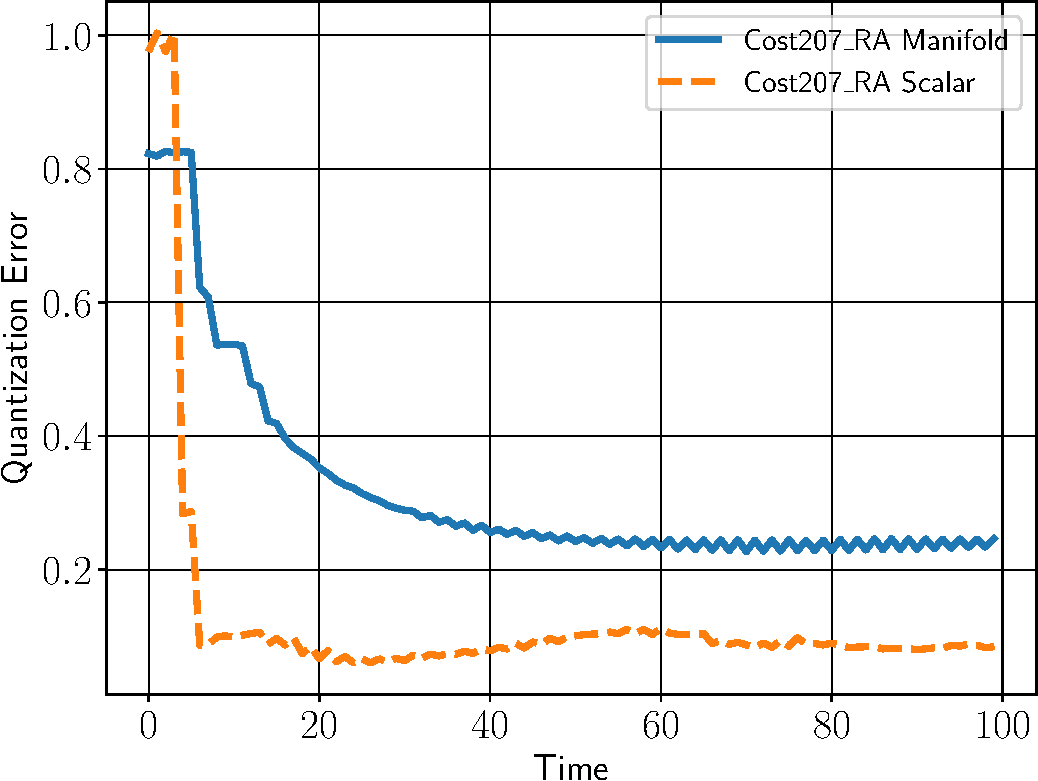
\includegraphics[width=\imwidth\columnwidth]{images/qerror.pdf}
\caption{\label{fig:error_decay}Comparison of the $4\times 2$
  precoder quantization error vs. time for the proposed
  approach (labelled ``Cost207\_RA Scalar'') and direct Stiefel
  manifold quantization (``Cost207\_RA Manifold'') for the COST207 channel.}
\end{center}
\end{figure}
This brings down the bit budget to an average of 5 bits for
$\bf{\Theta}$ and 5 bits for $\bf{\Phi}$ over alternate feedback
instances, thereby resulting in an average feedback budget of 5 bits,
as opposed to the 6 bits in~\cite{Gupt1905:Predictive}.

To enable adaptive tracking of the channel parameters, we start with
an initialization of the step size for each parameter, as discussed in
Equation~\ref{delta_eqn}. The value of $M$ was chosen to be $1.4$, and
can be adjusted appropriately to track the temporal evolution of
parameters for different Doppler frequencies.
\begin{figure}
% \begin{center}
\begin{subfigure}[b]{0.5\columnwidth}
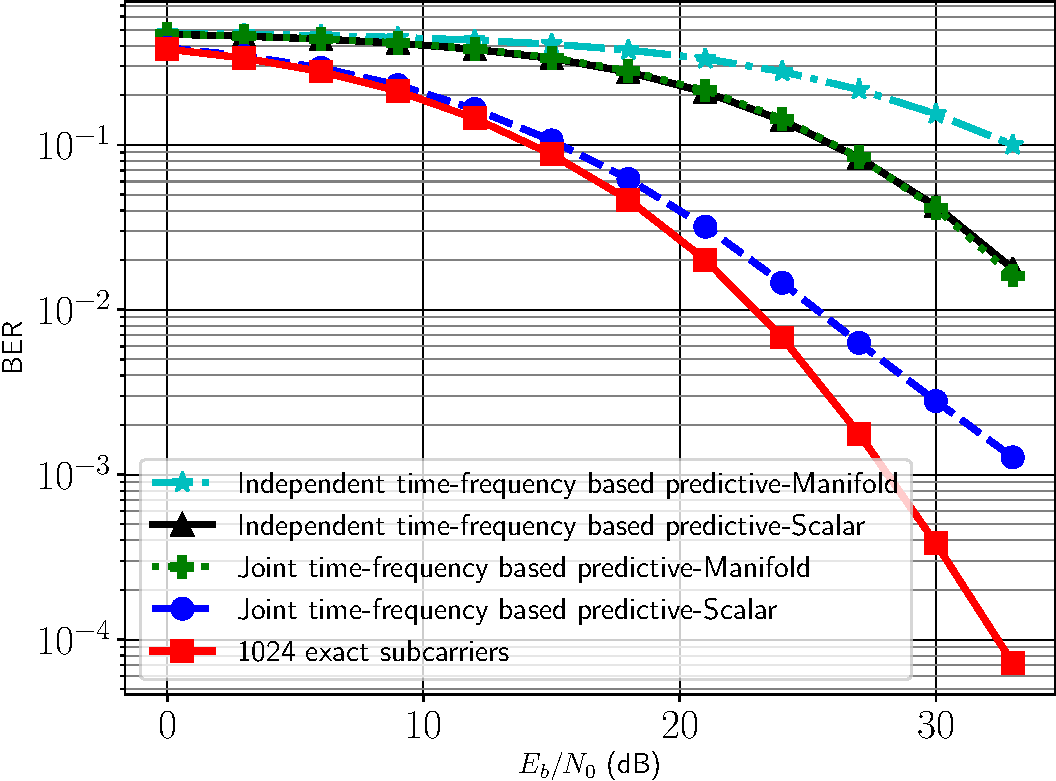
\includegraphics[width=\columnwidth]{images/1024final_withtime.pdf}
    \caption{}
\label{fig:ber_ped}
\end{subfigure}
\begin{subfigure}[b]{0.5\columnwidth}
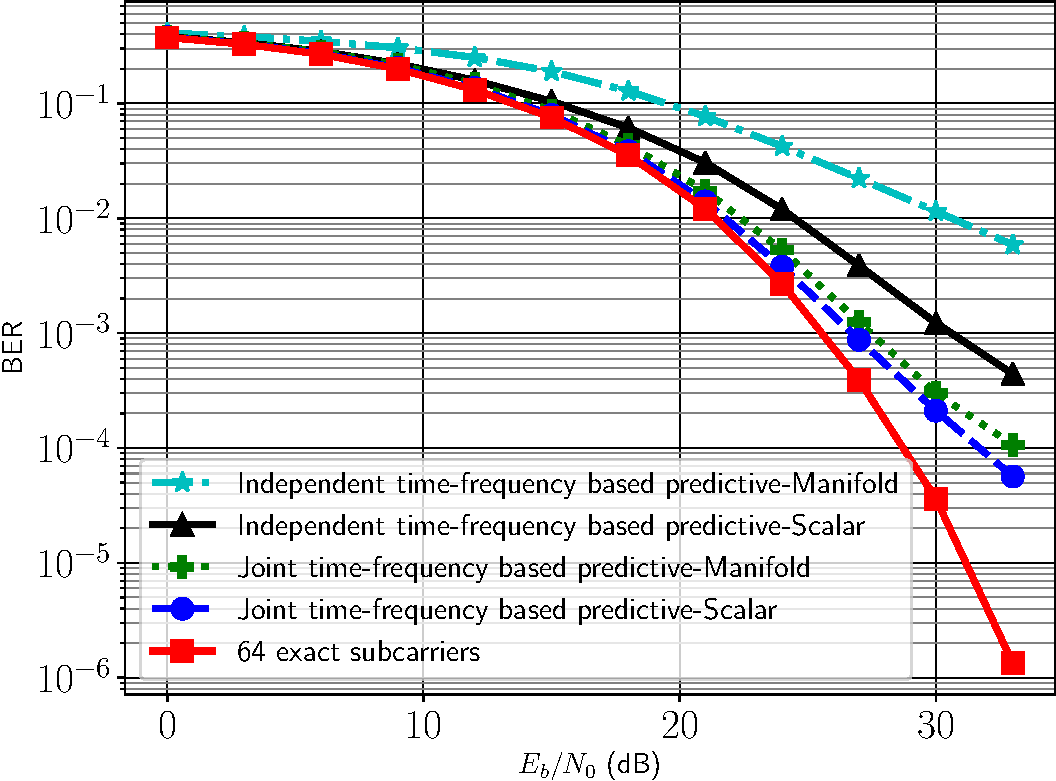
\includegraphics[width=\columnwidth]{images/64final_withtime.pdf}
\caption{}
% \caption{BER vs. SNR for QPSK transmission over the $4\times 2$ 64
%   subcarrier MIMO-OFDM system, with the ITU Cost207-RA channel profile
%   for $f_dT_s = 1.56\times 10^{-5}$, corresponding to a velocity of 172.8 km/h.}
\label{fig:ber_veh}
\end{subfigure}   
\caption{BER vs. SNR for QPSK transmission over the $4\times 2$
      MIMO-OFDM system, with the ITU Cost207-RA channel profile.
      a) 10244 subcarriers for $f_dT_s = 3.41\times 10^{-6}$, 
      corresponding to a velocity of 37.8 km/h. b) 64 subcarriers 
      for $f_dT_s = 1.56\times 10^{-5}$, 
      corresponding to a velocity of 172.8 km/h.
      }
% \end{center}
\end{figure}

\subsection{Results}
Fig.~\ref{fig:error_decay} shows the error decay rate with time for
the proposed approach and direct quantization on the Stiefel manifold
as described in~\cite{Gupt1905:Predictive}. Since the adaptation of
independent scalar parameters causes the error to decay rapidly, the
error is lower and the convergence is faster, even for larger starting
errors in the scalar quantization approach. The independence of the
parameters enables fast convergence. The Stiefel manifold based
approach with nested codebooks may thus be suboptimal when compared to
the parameterization using angles.

Fig.~\ref{fig:ber_ped} compares the BER obtained using the proposed
quantization method with that obtained using exact precoders for a
$4\times 2$ 1024 subcarrier system a slow fading
($f_dT_s = 3.41 \times 10^{-6}$). Independent time-frequency based
approaches correspond to the method without joint-time frequency
interpolation i.e. with prediction in time domain along with separate interpolation in the frequency domain.

We can observe that the performance of the proposed
method is close to the performance with exact precoders over a wide
range of SNRs. This can be attributed to the fact that even the 1-bit
update to the scalar parameters is able to approximate the precoder
very accurately. Since the channel variation across subcarriers is
gradual, owing to the limited delay spread of the channel profile,
linear interpolation and prediction yields good performance. Moreover,
this method outperforms the Stiefel manifold based approach since
adaptation of scalar parameters is more accurate than tangent space
based adaptation used over the Stiefel manifold. The obtained
performance moves closer to the optimal precoder when speeds reduce.
Also, similar to results shown in \cite{Gupt1905:Predictive}, the
joint time-frequency method outperforms the independent time-frequency
method, illustrating the benefits of exploiting joint correlations
versus just the independent correlations.

Fig.~\ref{fig:ber_veh} shows a similar comparison for a situation with
a higher speed. The faster variation of the channel taps with time
necessitates the use of a smaller number of subcarriers (viz. 64
subcarriers), thereby permitting more accurate tracking of precoders
on a per subcarrier basis. As in the previous case, we observe that
the scalar parameter-based approach outperforms manifold based
quantization by about 1 dB for higher SNRs. Since, on a per subcarrier
basis, the channel variation is slower, the precoder tracking is
better than the previous case. Faster channel variations would impose
limits on the efficacy of the proposed method in tracking the channel
parameters.

\section{Simulation 2}
\subsection{Simulation Setup}
For this scenario we consider an single user i.i.d Rayleigh MIMO channel with
$N_T$ transmitter antennas and $N_R$ receiver antennas. To study
the gain due to waterfilling we consider the case where $N_T=4$ 
and $N_R=2$. In the following results capacity gain is defined as
the percentage change in capacity of waterfilling case over non-waterfilling
case.

\subsection{Simulation Results}
Fig. \ref{fig:ccdf} shows CCDF plots of both waterfilling (WF)
and non-waterfilling (No-WF) scenarios at different SNRs. The plot is obtained by 
calculating capacity for 1000 different channel reaslizations. We can see that
with increasing SNR the gain due to WF reduces as SNR increases. This
is observed because at high SNRs, the optimal power distribution approaches
close to equal distribution.
\begin{figure}
\begin{center}
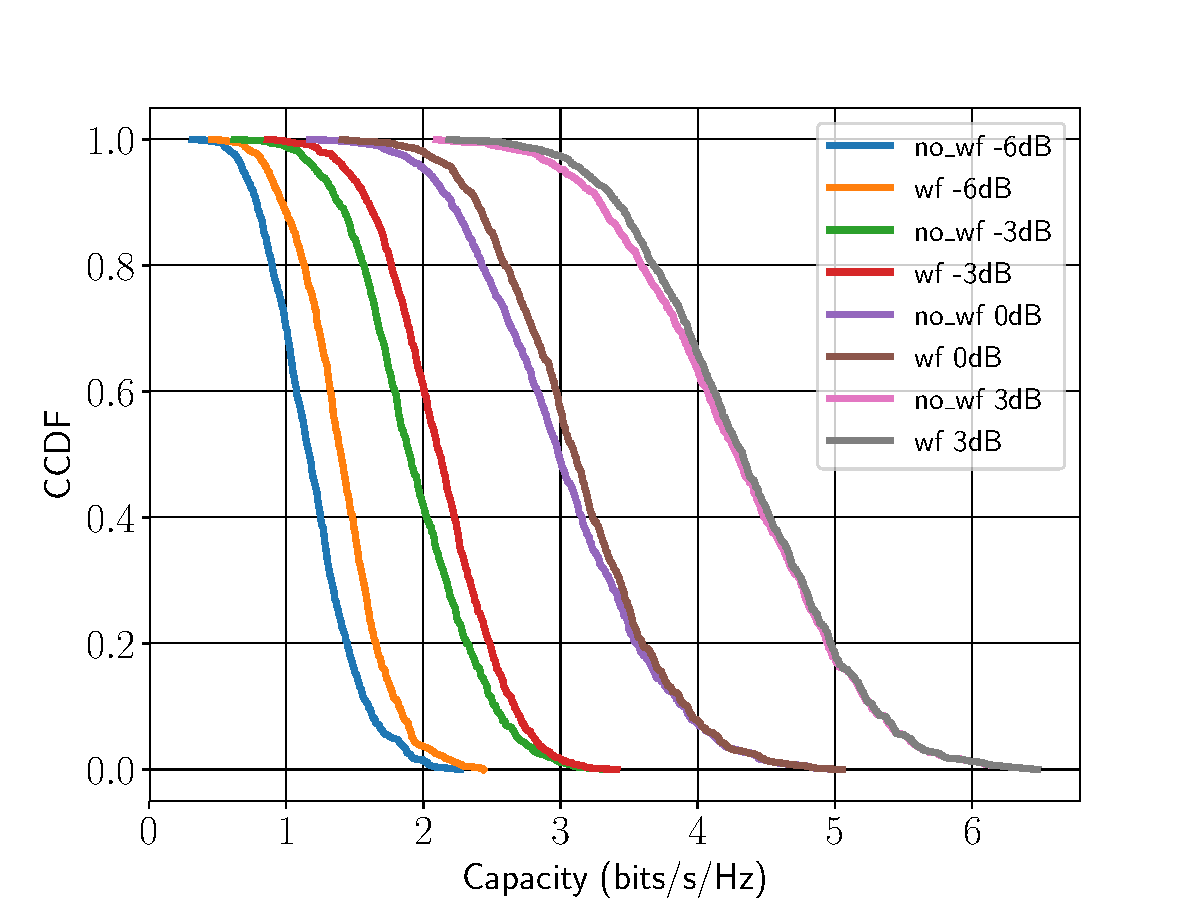
\includegraphics[width=\imwidth\columnwidth]{images/ccdf.pdf}
\caption{CCDF plots variation of $4\times2$ MIMO wireless channel i.e. $N_T=4$
and $N_R=2$ with different SNR values. Plots for both waterfilling and 
without waterfilling scenarios are compared.}
\label{fig:ccdf}
\end{center}
\end{figure}

In the following figures, capacity is calculated at $P_{out}=0.01$ (Outage Probability)
i.e. at $CCDF=99\%$.
In Fig.~\ref{fig:cap_gain} we can see that on increasing the number of transmitter
antennas the Capacity Gain$\%$ reduces. For $N_T=N_R=2$, it is as high as $50\%$
at -6dB SNR while it reduces to $20\%$ only for $N_T=6$. It reduces even further
for higher number of transmitters. It is observed because the difference between 
the eigen value decreases on increasing the number of transmitters which is
equivalent of distributing equal power among the transmitters from the Eq.~\ref{eq:lambda}.

In Fig.~\ref{fig:cap_vs_trans} capacity as $P_out=0.01$ is calculated for MIMO channel
with $N_R=2$ and varying number of transmitters. On increasing the number of transmitters
it can be seen that the difference between the capacity of WF and No-WF scenarios decreases.
The effect is even more pronounced at higher SNR which can be seen from the explanation
of Fig.~\ref{fig:cap_gain}.

\begin{figure}
\begin{center}
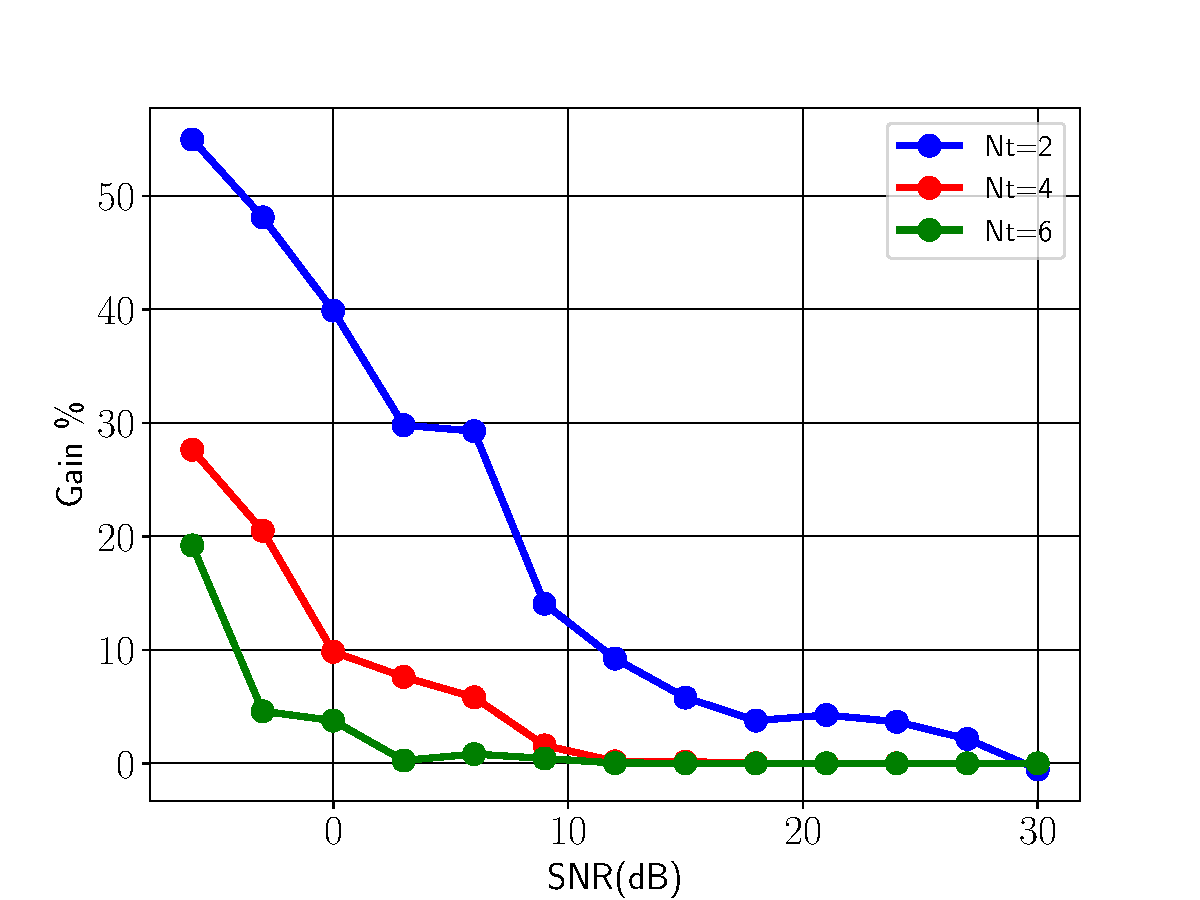
\includegraphics[width=\imwidth\columnwidth]{images/cap_gain.pdf}
\caption{Normalized capacity gain w.r.t no waterfilling situation with number
of receivers $N_R=2$ at $P_{out}=0.01$}
\label{fig:cap_gain}
\end{center}
\end{figure}

\begin{figure}
\begin{center}
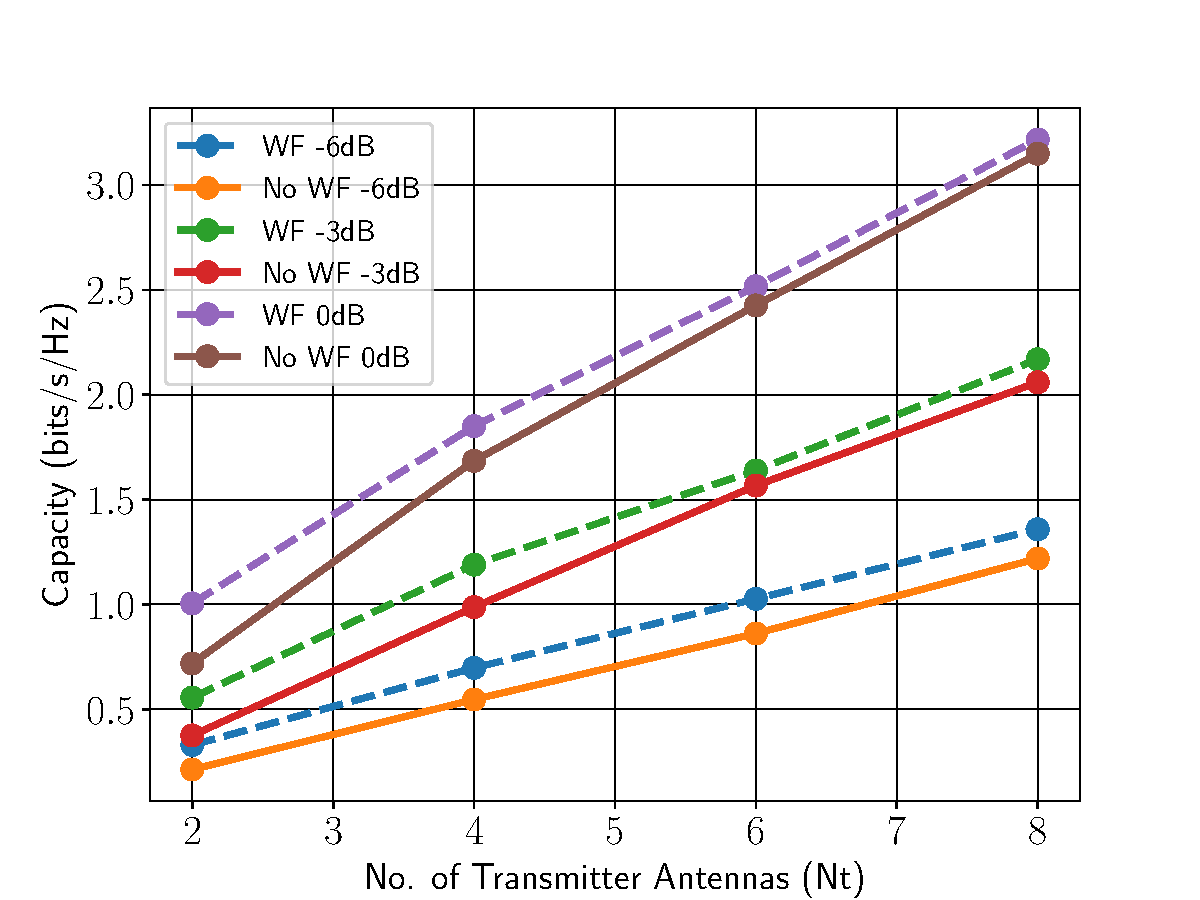
\includegraphics[width=\imwidth\columnwidth]{images/cap_vs_trans.pdf}
\caption{Variation of Capacity as a function of number of transmitters
    at $P_{out}=0.01$. Number of receivers is set constant at $N_R=2$.}
\label{fig:cap_vs_trans}
\end{center}
\end{figure}

\chapter{Conclusion and Future Work}
\subsection{Conclusion}
We have presented a predictive quantization based precoder
reconstruction for MIMO-OFDM systems that employs scalar quantization
based feedback of precoder parameters. Quantizing and adapting the
Givens rotation and Householder transformation parameters of precoders
minimizes receiver feedback to the transmitter while permitting
effective precoder adaptation. Exploiting temporal and frequency
correlations jointly enhances performance significantly. Simulations
reveal that the proposed approach converges faster and has smaller
errors when compared to manifold based approaches. Our feedback
approach, with simple 2D-interpolation over the scalar parameters,
tracks precoders effectively.

We have also showed that on increasing the number of transmitters (approaching towards Massive-MIMO scenario)
the difference between the capacities of WF and No-WF cases decreases.
Therefore, we can say that when channel has large number of transmitters
then precoder can be fed back to transmitter iteratively as shown in Chapter~\ref{chap:scheme}
and there is no need to feedback the singular values because equal power 
allocation provides similar results as compared to waterfilling.

\subsection{Future Work}
Future work would involve tuning the adaptation rates of scalar 
parameters and further reduction of redundancies to improve quantization.
Also currently in Massive-MIMO scenario lot of deep learning techniques have been 
used for limited CSI feedback and quantization. Therefore those techniques
can be studied and modified to obtain better results.
\bibliographystyle{ieeetr}
\bibliography{thesis}

\end{document}